\documentclass{homework}
\usepackage{lipsum}
\usepackage{cancel}
\usepackage{amsthm}
\usepackage{cleveref}
\usepackage{upgreek}
\usepackage{mathrsfs}
\usepackage{tikz}
\usepackage{units}
\newtheorem{lemma}{Lemma}

\DeclareMathOperator{\cov}{cov}

\title{Kevin Joyce}
\course{Stat 542 - Applied Linear Models - Homework 3}
\author{Kevin Joyce}
\docdate{\today}
\begin{document} 
\newcommand{\figref}[1]{\figurename~\ref{#1}}
\renewcommand{\bar}{\overline}
\renewcommand{\hat}{\widehat}
\renewcommand{\SS}{\mathcal S}
\newcommand{\HH}{\mathscr H}
\newcommand{\mom}{\widetilde}
\newcommand{\mle}{\widehat \Uptheta}
\newcommand{\eps}{\varepsilon}
\newcommand{\todist}{\stackrel{D}\longrightarrow}
\newcommand{\toprob}{\stackrel{p}\longrightarrow}
\newcommand{\TTheta}{\overline{\underline \Theta} }
\newcommand{\del}{\partial}
\newcommand{\approxsim}{\overset{\cdotp}{\underset{\cdotp}{\sim}}}
\newcommand{\RSS}{\ensuremath{\mathrm{RSS}}}
\newcommand{\MSE}{\ensuremath{\mathrm{MSE}}}
\newcommand{\SE}{\ensuremath{\mathrm{SE}}}
\newcommand{\TSS}{\ensuremath{\mathrm{TSS}}}
\newcommand{\SSReg}{\ensuremath{\mathrm{SSReg}}}
\problem{Faraway 3.1.}
For the \texttt{prostate} data, fit a model with \texttt{lpsa} as the response and the other variables as predictors.

\subproblem{ Compute 90 and 95\% CIs for the parameter associated with \texttt{age}.  Using just these intervals, what could we have deduced about the p-value for \texttt{age} in the regression summary?}

The 90\% CI for the age coefficient is (-0.0382,-0.0011), and the
95\% CI is (-0.0418,0.0026).  Since 0 is in the first but not the
second, we conclude that a two-sided $t$-test for $H_0\,:\beta_{age} = 0$
is between $.05$ and $.1$ providing moderate evidence of
significance.

%If, however, we use Bonferroni corrected margins of error, the respective joint 90 and 95\% CIs are (-0.0418,0.0026) (-0.0451,0.0058), and we conclude that the p-value for the joint significance test of the age parameter is greater than .1 yielding no evidence of significance.  

\subproblem{ Compute and display a 95\% joint confidence region for the parameters associated with \texttt{age} and \texttt{lbph}.  Plot the origin on this display.  The location of the origin on the display tells us the outcome of a certain hypothesis test.  State that test and its outcome.}

\begin{minipage}{.5\textwidth}
  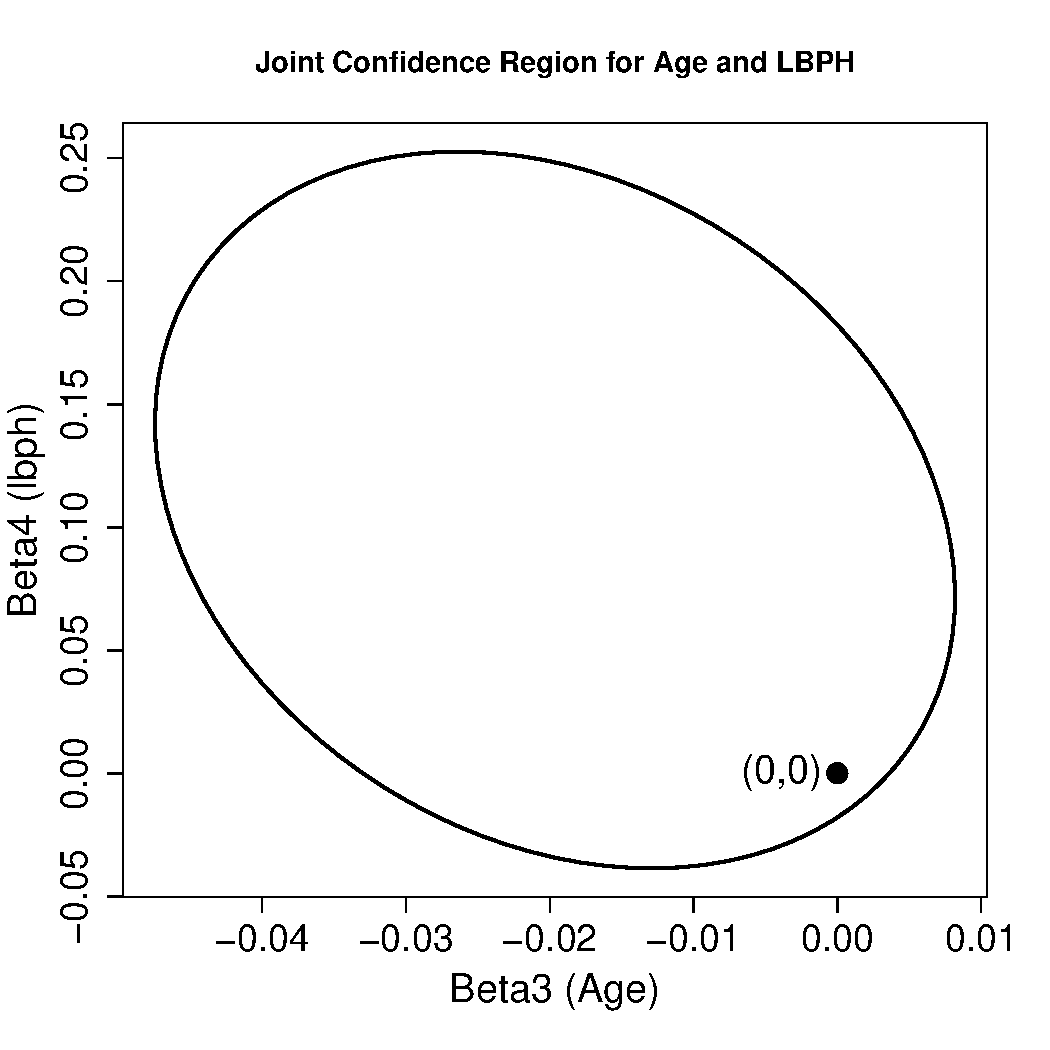
\includegraphics[width=\textwidth]{conf_region_1b.pdf}
\end{minipage}
\begin{minipage}{.5\textwidth}
  Whether the origin is within the confidence region tests the joint significance of age and lbph in the model - specifically, $H_0\,:\beta_3 = \beta_4 = 0$.  Since $(0,0)$ is within the region, we conclude (at $\alpha=.05$ level) that there is no statistical evidence to suggest that age and lbph are jointly significant in the model.
\end{minipage}

\subproblem{ Suppose a new patient with the following values arrives:\\
{\tt
\begin{tabular}{r r r r r r r r}
lcavol & lweight & age & lbph & svi & lcp & gleason & pgg45 \\
1.44692 & 3.62301 & 65.00000 & 0.30010 & 0.00000 & -0.79851 & 7.00000 & 15.00000\\
\end{tabular}\\
}
Predict the \texttt{lpsa} for this patient along with an appropriate 95\% CI.
} 

Let $\vect x_0$ be the $1\times p$ vector of values given in the table above (with a one prepended). Then the 95\% CI is given by 
$$
  \vect x_0 \vect{\hat \beta} \pm t_{.975}(n-p)\sqrt{\MSE\cdot\vect x_0'(\vect{X'X})\vect x_0} \approx 2.389\pm 0.217
\text{ or }
( 2.172, 2.606 ). $$

\subproblem{ Repeat the last question for a patient with the same values except that he or she is age 20.  Explain why the CI is wider. }

In this case, let $\vect x_1$ denote the explanatory variables, then
$$
  \vect x_1 \vect{\hat \beta} \pm t_{.975}(n-p)\sqrt{\MSE\cdot\vect x_1'(\vect{X'X})\vect x_1} \approx 3.272 \pm 1.012
\text{ or }
( 2.260, 4.285 ). $$


\begin{minipage}{.3\textwidth}
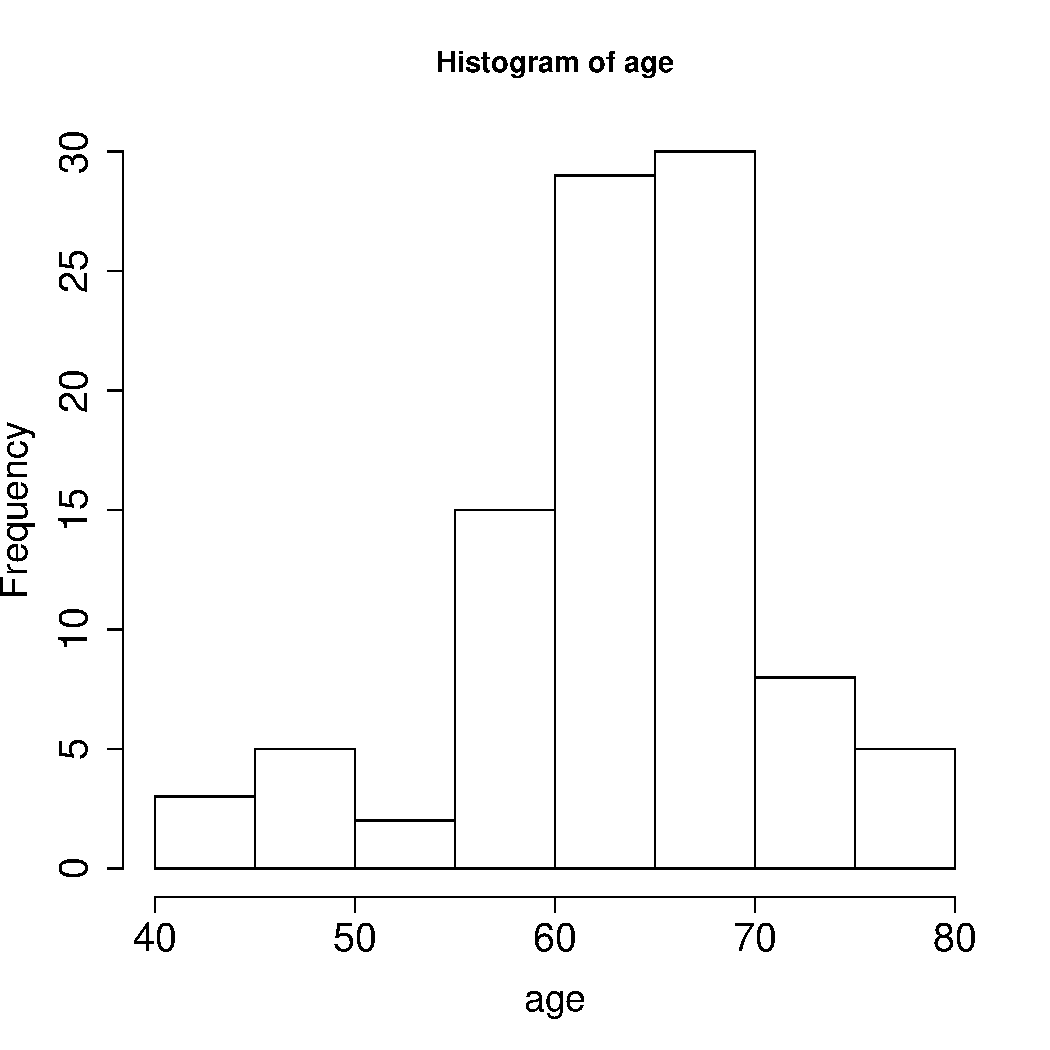
\includegraphics[width=\textwidth]{age_hist.pdf}
\end{minipage}
\begin{minipage}{.7\textwidth}
The increase in uncertainty is due to the lack of data points for ages near 20.  This is evident in the histogram of ages to the left.
\end{minipage}

\subproblem{ In the text, we made a permutation test corresponding to the $F$-test for the significance of all the predictors.  Execute the permutation test corresponding to the $t$-test for age in this model.  (Hint: \texttt{summay(g)\$coef[4,3]} gets you the $t$-statistic you need if the model is galled \texttt g.)}

We fit the model with 4999 permutations of the age variable and compare the $F$-statistic given by squaring the $t$-statistic for the age coefficient and compare it to the unpermuted coefficient via the codes
{\small
\begin{verbatim}
nperm = 4999
F1 = mdl$coef[4,3]
numerator = sum(replicate(nparm, 
    summary(lm(lpsa~lcavol+lweight+sample(age)+lbph+svi+lcp+gleason+pgg45))$coef[4,3]^2 > F1
  ))
(p = (numerator+1)/(nperm+1)) 
\end{verbatim}
}
This resulted in the p-value of 0.0814, providing slight evidence for significance.

\problem{Faraway 3.3.}
Using the \texttt{teengamb} data, fit a model with \texttt{gamble} as the response and the other variables as predictors.  

\subproblem{ Which variables are statistically significant? }

In the full model, the Coefficients Table reports:
{\small\begin{verbatim}
Coefficients:
             Estimate Std. Error t value Pr(>|t|)    
(Intercept)  22.55565   17.19680   1.312   0.1968    
sex         -22.11833    8.21111  -2.694   0.0101 *  
status        0.05223    0.28111   0.186   0.8535    
income        4.96198    1.02539   4.839 1.79e-05 ***
verbal       -2.95949    2.17215  -1.362   0.1803    
\end{verbatim}}
This indicates that sex and income are significant in the model with each predictor.

\subproblem{ What interpretation should be given to the coefficient for \texttt{sex}?}

Since the sex codes are 0=male and 1=female, we conclude that holding all other predictors constant, on average males gambled about \pounds22 more a week than females.

\subproblem{ Predict the amount that a male with average (given these data) status, income, and verbal score would gamble along with an appropriate 95\% CI.  Repeat the prediction for a male with maximal values (for this data) of status, income and verbal score.  Which CI is wider and why is this result expected? }

The average male predictor is given by $\vect{\bar x_{m}} \approx ( 1,0, 45.234 , 4.642 , 6.660 )'$, and the 95\% CI for its gambling expenditure is given by
$$
 \vect{\bar x_{m}}'\vect{\hat \beta} \pm t_{.975}(n-p)\sqrt{\MSE\cdot\vect {\bar x_m}'(\vect{X'X})\vect {\bar x_m}}\approx 28.24\pm9.46\text{ or }(18.78,37.70).
$$

\subproblem{ Fit a model with just \texttt{income} as a predictor and use an $F$-test to compare it to the full model. }

The ANOVA model comparison test gives
$$
  F = \frac{\RSS_\omega - \RSS_\Omega}{\MSE} \approx 4.134\quad\text{ and }\quad p = 0.012.
$$
So, there is some statistical evidence that sex, status, and verbal score add explanatory significance to the model.

\problem{Faraway 3.4.}
Using the \texttt{sat} data:

\subproblem{ Fit a model with \texttt{total} sat score as the response and \texttt{expend, ratio} and \texttt{salary} as predictors.  Test the hypothesis that $\beta_{salary} = 0$.  Test the hypothesis that $\beta_{salary} = \beta_{ratio} = \beta_{expend} = 0$. Do any of these predictors have an effect on the response? }

\begin{minipage}{.6\textwidth}
{\small \begin{verbatim}
Coefficients:
            Estimate Std. Error t value Pr(>|t|)    
(Intercept) 1069.234    110.925   9.639 1.29e-12 ***
expend        16.469     22.050   0.747   0.4589    
ratio          6.330      6.542   0.968   0.3383    
salary        -8.823      4.697  -1.878   0.0667 .  
---
Signif. codes:  0 ‘***’ 0.001 ‘**’ 0.01 ‘*’ 0.05 ‘.’ 0.1 ‘ ’ 1 

Residual standard error: 68.65 on 46 degrees of freedom
Multiple R-squared: 0.2096,     Adjusted R-squared: 0.1581 
F-statistic: 4.066 on 3 and 46 DF,  p-value: 0.01209 
\end{verbatim}}
\end{minipage}
\begin{minipage}{.4\textwidth}
From the \texttt{summary} command on the linear model, we test $H_0\,:\beta_{salary} = 0$ and see that $\beta_{salary}$ marginally significant ($p = 0.0667$) in the full model. The test for model significance, $H_0\,:\beta_{salary} = \beta_{ratio} = \beta_{expend} = 0$, also provides marginal evidence contrary to $H_0$ - that is, there is statistical evidence suggesting significant explanatory power of the model. We note the sample size is 50, and thus the statistical significance may not be pratically significant especially in the absence of a scientific explanation. 
\end{minipage}

\subproblem{Now add \texttt{takers} to the model.  Test the hypothesis that $\beta_{takers} = 0$.  Compare this model to the previous one using an $F$-test.  Demonstrate that the $F$-test and $t$-test here are equivalent.}

\begin{minipage}{.6\textwidth}
{\small \begin{verbatim}
Coefficients:
             Estimate Std. Error t value Pr(>|t|)    
(Intercept) 1045.9715    52.8698  19.784  < 2e-16 ***
expend         4.4626    10.5465   0.423    0.674    
ratio         -3.6242     3.2154  -1.127    0.266    
salary         1.6379     2.3872   0.686    0.496    
takers        -2.9045     0.2313 -12.559 2.61e-16 ***
...
> anova(mdl2,mdl) 
Analysis of Variance Table

Model 1: total ~ expend + ratio + salary + takers
Model 2: total ~ expend + ratio + salary
  Res.Df    RSS Df Sum of Sq      F    Pr(>F)    
1     45  48124                                  
2     46 216812 -1   -168688 157.74 2.607e-16 ***
\end{verbatim}}
\end{minipage}
\begin{minipage}{.4\textwidth}
Note that the percentage of those elligable to take the test is highly significant in the full model with a p-value of $2.61\times10^{-16}$. The $t$-test and $F$-test produce an identical p-value.  In fact,
{\footnotesize \begin{verbatim}
> anova(mdl2,mdl)[2,5] - summary(mdl2)$coefficients[5,3]^2 
[1] 0
\end{verbatim}
}

\end{minipage}

\newpage
\begin{longproblem}
  For each of the following regression models, indicate whether it is a general linear regression model. If it is not, state wheter it can be expressed in the general linear model form:
$$
  y_i = \beta_0 + \beta_1 x_{i1} + \dots + \beta_{p-1}x_{i,p-1} + \epsilon_i
$$

\subproblem{$y_i = \beta_0 + \beta_1 x_{i1} + \beta_2 \log_{10} x_{i2} + \beta_3x_{i1}^2 + \epsilon_i$}

This \emph{is} a linear regression model.

\subproblem{$y_i = \epsilon_i\exp(\beta_0 +\beta_1 x_{i1} +\beta_2x_{i2}^2$}

If we log-transform the response, then we have the general linear regression model
$$
  \log y_i = \beta_0 +\beta_1 x_{i1} +\beta_2x_{i2}^2 + \log \epsilon_i.
$$

\subproblem{$y_i = \beta_0 + \log_{10}(\beta_1 x_{i1}) + \beta_2 x_{i2} + \epsilon_i$}

This problem is \emph{not} linear due to the term $\log_{10}(\beta_1 x_{i1})$, and there is no obvious transformation that will make the model linear.

\subproblem{$y_i = \beta_0\exp(\beta_1x_{i1}) + \epsilon_i $} 

This problem is also \emph{not} linear due to the term $\beta_0\exp(\beta_1x_{i1})$, and a log transformation will not work as in (b) since the error is additive.

\subproblem{$y_i = [1+\exp(\beta_0 +\beta_1 x_{i1} +\beta_2x_{i2}^2+\epsilon_i)]^{-1}$}

Consider the transformation $g(y) = \log (y^{-1} - 1)$.  Then, the transformed model is
$$
  g(y_i) = \beta_0 +\beta_1 x_{i1} +\beta_2x_{i2}^2+\epsilon_i,
$$
which is a general linear regression model.
\end{longproblem}

\begin{longproblem}
The information below relates a response variable $y$, a second measurement on
wood volume, to four explanatory variables defined as: $x_1 = $ a first
measurement on wood volume, $x_2 = $ the number of trees, $x_3 = $the average
age of trees, and $x_4 = $ the average volume per tree.  Note that $x_4 =
x_1/x_2$.  Some of the information in the coefficients table and Analysis of
Variance table below has not been reported, so that you can figure it out on
your own.

{\small
\begin{minipage}{.45\textwidth}
\begin{tabular}{c c c c c}
\multicolumn{5}{c}{\bf Coefficients Table} \\ \hline
Predictor & $\hat \beta_k$ & $\mathrm{SE}(\hat \beta_k)$ & $t$ & p-val \\ \hline
Intercept & 23.45   & 14.90   &        & 0.122 \\
$x_1$     & 0.93209 & 0.08602 &        & 0.000 \\ 
$x_2$     &         & 0.4721  & 1.5554 & 0.126 \\
$x_3$     &-0.4982  & 0.1520  &        & 0.002 \\
$x_4$     &3.486    &2.274    &        & 0.132 \\ \hline
\end{tabular}
\end{minipage}
\begin{minipage}{.45\textwidth} 
\begin{center}
\begin{tabular}{c c c c c c}
\multicolumn{6}{c}{\bf Analysis of Variance Table}\\
\hline
Source & df & SS & MS & F & p-val\\ \hline
Regression & 4 & 887994 &  &  & 0.000 \\
Error & & & & & \\
Total & & 902773 & 16718.02 & & \\ \hline
\end{tabular}
\begin{tabular}{c c c}
\multicolumn{3}{c}{\bf Sequential Sums of Squares}\\ \hline
Source & df & Seq. SS \\ \hline
$x_1$& 1 & 883880 \\
$x_2$& 1 & 183 \\
$x_3$& 1 & 3237 \\
$x_4$& 1 & 694\\\hline
\end{tabular}
\end{center}
\end{minipage}
}

\subproblem{How many observations are in these data?}

$$n = \TSS/\mathrm{MST} + 1 = (902773/16718.02) + 1 = 55.$$

\subproblem{What is $R^2$ for this model?}

$R^2$ is given by the regression sum of squares ($\mathrm{SSReg}$) over the total sum of squares (TSS).  From the partial ANOVA table we calculate
$$
  \frac{\SSReg}{\TSS} = \frac{887994}{902773} \approx 0.9836.
$$

\subproblem{ What is the mean squared error? }

$$
  \mathrm{MSE} = \frac{\mathrm{RSS}}{n-p} = \frac{\TSS-\SSReg}{n-p} = \frac{902773 - 887994}{55 - 5} = 295.58
$$

\subproblem{ Give a 95\% confidence interval for $\beta_2$.}

 The $t$-statistic in the Coefficients Table tests if the coefficient is $0$, hence, is given by
$$
   t^* = \frac{\hat \beta_2}{\mathrm{SE}(\hat \beta_2)} \iff \hat \beta_2 = \mathrm{SE}(\hat \beta_2)\cdot t^* \approx 0.4721\cdot1.5554 \approx0.734 .
$$
The confidence interval (with Bonferroni correction) is of the form 
$$\hat \beta_2 \pm t_{1-0.5/(2\cdot5)}(50)\cdot\mathrm{SE}(\hat \beta_2) \approx0.734 \pm 1.264.\text{ or }( -0.530, 1.998 )$$

\subproblem{ Test the null hypothesis $H_0\,:\,\beta_3 = 0$. }

The fourth row of the Coefficients Table tests this hypothesis, and the reported p-value is 0.002 which gives fairly strong evidence that the coefficient is 0.

\subproblem{ Test the null hypothesis $H_0\,:\,\beta_1 = 1$. Why might this hypothesis be of interest?} 

We calculate 
$$
  t^* = \frac{\hat \beta_1 - 1}{\mathrm{SE}(\beta_1)} \approx -0.789
$$
and calculate the p-value for two-sided test $p = 2P(t \le t^*)
\approx 0.434$.  Hence, we conclude that there is no evidence to suggest that $\beta_1 \not= 1$.  This is not surprising since $x_1$ was a second measurement of the response.  In some sense, this test indicates that the methods for measuring the response and second measurement agree.

\subproblem{ Give the F-statistic for testing $H_0\,:\,\beta_3 = 0$ relative to the full model.}

It can be shown [Renchner 204-205 and HW1.8a] that the $F$-statistic is given by squaring the associated $t$-statistic from the Coefficients Table. I.e.
$$
  F = t^2 = \left(\frac{\hat\beta_3}{\SE(\hat\beta_3)}\right)^2 = \left(\frac{-0.4982}{0.1520}\right)^2 = 10.74287.
$$
%$$
%  F = \frac{\mathrm{SSReg}(x_3|x_1,x_2,x_4)}{\MSE(x_1,x_2,x_3,x_4)} = \frac{\SSReg(x_1,x_2,x_3,x_4)}{fuck}
%$$

\subproblem{ Give $R(\beta_3|\beta_1,\beta_2)$ and find $R(\beta_3|\beta_1,\beta_2,\beta_4)$.}

From the Sequential Sums of Squares table, we can read directly
$$
  R(\beta_3|\beta_1,\beta_2) = \SSReg(x_3|x_1,x_2) = 3237.
$$
On the other hand, we can recover $R(\beta_3|\beta_1,\beta_2,\beta_4)$ from the
$F$-statistic calculated in (g). That is, 

$$
F = \frac{R(\beta_3|\beta_1,\beta_2,\beta_4)}{\MSE} \iff R(\beta_3|\beta_1,\beta_2,\beta_4) = \MSE\cdot F \approx 295.58\cdot10.74287\approx3175.377
$$

\newpage
\subproblem{ Test the model with only variables $x_1$ and $x_2$ against the model with all of the variables $x_1,x_2,x_3,x_4$.}

The relavant $F$-statistic is
$$
  F = \frac{\SSReg(x_1,x_2)/2}{\MSE(x_1,x_2,x_3,x_4)}= \frac{(\SSReg(x_1) + \SSReg(x_2|x_1))/2}{\MSE(x_1,x_2,x_3,x_4)} = \frac{(883880+8183)/2}{295.5} = 1495.471.
$$
The p-value for the test is practically 0 since $F \gg 1$, hence significant evidence exists for the joint explanatory power $x_1$ and $x_2$.  

\subproblem{ Test the model with only variables $x_1$ and $x_2$ against the model with variables $x_1,x_2,$ and $x_3$. }

Note that $\RSS(x_1,x_2,x_3) = \RSS(x_1,x_2,x_3,x_4) + \SSReg(x_4|x_1,x_2,x_3) = 15473$.  Hence the relavant $F$-statistic is

$$
  F = \frac{\SSReg(x_1,x_2)/2}{\RSS(x_1,x_2,x_3)/(n-p+1)} = \frac{(883880+8183)/2}{14085/51} = 1456.964.
$$
As before, the p-value is practically 0 providing significant evidence for the joint significance of $x_1$ and $x_2$.

\subproblem{ Should the test in part (g) be the same as the test in part (j)?  Why or why not?}

These are distinct tests (note the different $F$-statistics). The first tests the significance of
$x_1,x_2$ in the context of the full model with $x_1,x_2,x_3,x_4$,
while the second tests only relative to $x_1,x_2$, and $x_3$.  Although, since the coefficient for $x_4$ is not significant ($p = .123$), the competing explanatory power gained by droping $x_4$ was marginal. Hence there are similar $F$-statistics in each case.


\subproblem{ For estimating the point on the regression surface at $(x_1,x_2,x_3,x_4) = (100,25,50,4)$, the standard error of the estimate for the point on the surface is 2.62.  Give the estimated point on the surface, a 95\% confidence interval for the point on the surface, and a 95\% prediction interval for a new point with these $x$-values.}

The prediction is given by 
$$
  \hat{ y|\vect x_0} = (1,100,25,50,4) \hat{\vect\beta} \approx  124.0506.
$$
 The 95\% CI for the mean response given $\vect x_0' = (1,100,25,50,4)$ is
given by 
$$\hat{ y|\vect x_0} \pm t_{.975}(n-p)\cdot\SE(\hat{y|\vect x_0}) \approx 124.051 \pm 5.262\text{ or }(
118.788, 129.313 ).$$  
Since $\SE(\hat{y|x_0}) = \sqrt{\MSE \cdot\vect{x_0'(X'X)^{-1}x_0}}$,the prediction interval is given by 
$$\hat{ y|\vect x_0} \pm t_{.975}(n-p)\sqrt{\MSE\cdot(1+\SE(\hat{y|x_0})^2/\MSE)}\approx 124.051 \pm 34.93$$
$$\text{ or }( 89.120, 158.981 ).$$
 

\subproblem{ Test the null hypothesis $H_0\,:\,\beta_1=\beta_2=\beta_3=\beta_4=0$. }

This is the model significance test given by the $F$-statistic
$$
  F = \frac{(\TSS - \RSS)/(p-1)}{\MSE} \approx 751.0606,
$$
Which yields a p-value that is practially 0.  Hence, the model is significant.
\end{longproblem}

\begin{longproblem}
A random sample of 20 incomping shipments of chemicals in drums arriving at a warehouse was taken where measurements were taken on the number of drumps in the shipment $(x_1)$, the total weight of the shipment in hundreds of pounds $(x_2)$, and the number of minutes required to handle the shipment $(y)$. The data are given in three columns in the same order as above in the file \texttt{shipment.txt} on the course web page.

\subproblem{ Using matrix notation, fit the model:
$$
  y_i = \beta_0 +\beta_1 x_{i1} + \beta_2 x_{i2} + \epsilon_i,\quad i = 1,\dots,n,\quad \epsilon_i \stackrel{iid}{\sim} N(0,\sigma^2).
$$ 
Report the following vectors and matrices: $\vect{X'X}, \vect{X'y}, \vect{y'y}, (\vect{X'X})^{-1}, \&\, \vect{\hat \beta} = (\vect{X'X})^{-1} \vect{X'y}$.
}

The model in matrix form is

$$
\vect y = \vect X \vect \beta + \vect \epsilon,
$$
where $\vect y$ and $\vect \epsilon$ are $n \times 1$ with entries $y_i$ and $\epsilon_i$ respectivly, $\vect X$ is $n\times 3$ with entries $x_{ij}$ with $j=0,1,2$, and $\beta$ is $3 \times 1$ with entries $\beta_j$.  The following table summarizes the desired matrix computations.

\renewcommand{\arraystretch}{1.2}
\begin{center}
\begin{tabular}{|c c c c c|}
$\vect{X'X}$ & $\vect{X'y}$ & $\vect{y'y}$ & $(\vect{X'X})^{-1}$ & $(\vect{X'X})^{-1} \vect{X'y}$ \\\hline
$ 
\begin{bmatrix}
 20.00 &  238.00 &  182.240\\
238.00 & 3420.00 & 2671.060\\
182.24 & 2671.06 & 2161.227\\
\end{bmatrix}
$ & $
\begin{bmatrix}
 1889.00 \\
27246.00 \\
21648.81 \\
\end{bmatrix}
$ &
219449
& $
\begin{bmatrix}
 0.307& -0.033&  0.015\\
-0.033&  0.012& -0.012\\
 0.015& -0.012&  0.014\\
\end{bmatrix}
$ & $
\begin{bmatrix}
3.324\\
3.768\\
5.080\\
\end{bmatrix}
$
\end{tabular}
\end{center}

\subproblem{Estimate the variance-covariance matrix of the vector $\vect{ \hat \beta}$.}

$$
\hat{\mathrm{Var}(\vect{\hat \beta})} = (\vect{X'X})^{-1}\cdot\MSE \approx
\begin{bmatrix}
 9.677 & -1.040 &  0.469\\
-1.040 &  0.377 & -0.379\\
 0.469 & -0.379 &  0.443\\
\end{bmatrix}.
$$
\subproblem{Test whether or not $\beta_2 > 50$ and interpret your conclusion clearly in the language of the problem. }

We test $H_0:\,\beta_2 \le 50$. The test statistic is

$$
  t^* = \frac{ \hat \beta_2 - 50 }{ \SE(\hat \beta_2) } \approx -67.49392.
$$
Hence $P( t > t^* ) \approx 1$ and we conclude that there is an extreme lack of
evidence for ${H_a:\,\beta_2 > 50}$. Practically, given that $\hat \beta_2
\approx 5.08$ and $SE(\hat \beta_2)^2 = 0.433$, we have absolutely no reason to believe
that a shipment weighing 100 more pounds will result in more than 50 minutes of
handling time (fixing the amount of drums). 
\newpage

\newcommand{\Var}{\mathrm{Var}}
\subproblem{ Noting that for random variables $U,V$ and constants $a,b$, we have:
$$
  \Var(aU + bV) = a^2\Var(U) + b^2\Var(V) + 2ab\mathrm{Cov}(U,V),
$$
compute the standard error of $\hat \beta_1 + 2\hat \beta_2$ using part (b) above, and test whether or not $\beta_1 = -2\beta_2$.}

From above,
$$
  \Var(\hat \beta_1 + 2\hat \beta_2) = \Var(\hat\beta_1) + 4\Var(\hat\beta_2) + 4\mathrm{Cov}(\beta_1,\beta_2).
$$
Hence, an estimate for $\sqrt{\Var(\hat\beta_1 + 2\hat \beta_2)}$ is
$$
  \SE(\hat \beta_1 + 2\hat \beta_2) = \sqrt{ \hat{\Var(\vect{\hat \beta})}_{22} + 4\hat{\Var(\vect{\hat \beta})}_{33} + 4\hat{\Var(\vect{\hat \beta})}_{2,3} } \approx 0.7967.
$$
Note that $\hat \beta_1 + 2\hat \beta_2 \sim N(\beta_1 + 2\beta_2,\Var(\hat\beta_1 + 2\hat \beta_2))$. Hence, we can test $H_0:\,\beta_1 + 2\beta_2 = 0$ with the $t$-statistic 
$$
t^* = \frac{\hat \beta_1 + 2\hat \beta_2}{\SE(\hat \beta_1 + 2\hat \beta_2)} \approx 17.482,
$$
with p-value $2P(t > |t^*|) \approx 0$.  Hence, there is fairly significant evidence to conclude ${\beta_1 \not= -2\beta_2}$.

\subproblem{Find a 90\% confidence interval for $\beta_1 + 2\beta_2$.}

The confidence interval is given by
$$
  \hat \beta_1 + 2\hat \beta_2 \pm t_{.95}(n-p)\SE(\hat \beta_1 + 2\hat \beta_2) \approx 13.927 \pm 1.386\text{ or }( 12.541,15.313 ).
$$

\end{longproblem}

\begin{longproblem}
Thinning of the protective layer of ozone surrounding the earth may have catastrophic consequences.   A team of University of California scientists estimated that increased solar radiation through the hole in the ozone layer over Antarctica altered processes to such an extent that primary production of phytoplankton was reducec 6-12\%.

Depletion of the ozone layer allows themost damaging ultraviolet raidation - UVB (\unit[280-320]{mm}) - to reach the earth's surface.  An important consequence is the egree to which oceanic phytoplankton production is inhibited by exposure to UVB, both near the ocean surface (where the effect should be slight) and below the surface (where the effect could be considerable).

To measure this relationship, the researchers sampled from the ocean column at various depths at 17 locations around Antarctica during the austral spring of 1990.  To account for shifting of the ozone hole's positioning, they considered a measure of UVB exposure integrated over exposure time.  The exposure measurements and the percentage of inhibition of normal phytoplankton production were extracted from their graph to produce the data in the file \texttt{ozone.txt} on the course webpage.  These data contain 4 variables: the location number, percent inhibition, UVB exposure, and depth of measurement (S=surface, D=deep).

Does the effect of UVB exposure on the distribution of percentage inhibition differ at the surface and in the deep?  How much difference is there?  Analyze these data and write a summary of statistcal findings in no more than one page.  (Suggestion: Fit the model with different intercepts and different slopes, even if some terms are not significantly different from zero.)
\end{longproblem}
\end{document} 
